\documentclass[12pt,a4paper]{exam}

% --------------------
% Packages
% --------------------
\usepackage[utf8]{inputenc}
\usepackage[T1]{fontenc}
\usepackage[french]{babel}
\usepackage{amsmath,amssymb}
\usepackage{geometry}
\usepackage{tikz}
\usetikzlibrary{angles,quotes}
\usetikzlibrary{calc}
\usepackage{pgfplots}
\pgfplotsset{compat=1.18}
\geometry{margin=2cm}

% Pour les coordonnées de vecteurs :
\newcommand*{\Coord}[2]{%
  \ensuremath{
    \begin{pmatrix}
      #1 \\[0pt]
      #2
    \end{pmatrix}}
}

% --------------------
% En-tête / pied (exam)
% --------------------
\header{\textbf{NOM Prénom : }}{}{2\up{nde}}
\footer{}{\thepage}{}

% --------------------
\begin{document}

\begin{center}
    \Large\textbf{Devoir Surveillé\\Droites du plan et vecteurs}
\end{center}

\vspace{0.3cm}

\noindent
\textbf{Durée :} 1h \hfill
\textbf{Calculatrice :} \underline{NON} autorisée

\vspace{0.5cm}

% ========================================================
%             Exo : graphique
% ========================================================
\noindent
\textbf{Exercice 1 : Des droites (\ \ \ \  / 4 points )}

\vspace{10pt}
On considère le graphique ci-dessous :

\begin{center}
    \begin{tikzpicture}[scale=1]
    \begin{axis}[
        width=9cm,
        height=9cm,
        axis lines=center,
        grid=both,
        xmin=-2, xmax=6,
        ymin=-4, ymax=4,
        % xtick={-4,-3,-2,-1,0,1,2,3,4},
        % ytick={-4,-3,-2,-1,0,1,2,3,4},
        samples=200,
    ]
    \addplot[domain=-2:6, thick] {(2/3)*x - 3};
    \node at (axis cs:4.5,0.5) {$(d_1)$};
    \end{axis}
    \end{tikzpicture}
\end{center}


\begin{questions}

\question[2] Déterminer l'équation cartésienne de la droite $(d_1)$.

\question[1] Tracer sur ce graphique la droite $(d_1)$ d'équation $y +x -2 = 0$.

\question[1] Tracer la droite d'équation $x = \dfrac{5}{2}$.

\end{questions}

\vspace{1cm}

% ========================================================
%             Exercice 2
% ========================================================
\noindent
\textbf{Exercice 2 : Un peu plus compliqué ( \ \ \ / 6 points )}

\vspace{10pt}
Dans un repère orthonormé $(O;\overrightarrow{i};\overrightarrow{j})$, on considère les points 
$A\Coord{-3}{5}$, $B\Coord{9}{2}$ et $C\Coord{2}{0}$.

\begin{questions}

\question[2] Déterminer une équation cartésienne de la droite $(AB)$.

\question[2] Montrer que le point $C$ n'appartient pas à la droite $(AB)$.

\question[2] Déterminer une équation cartésienne de la droite $(d)$ passant par $C$ et de coefficient 
directeur $\dfrac{7}{2}$.

\end{questions}

\vspace{2cm}

\begin{center}
    \underline{\textbf{Retourner le sujet}}
\end{center}


\newpage
% ========================================================
%             Exercice 3 : placer un 2 points à l'aide de relations vectorielles (chasles?)
%               et 
% ========================================================
\noindent
\textbf{Exercice 3 : Encore un parallélogramme... ( \ \ \ / 6 points )}

\vspace{10pt}
On considère le tracé suivant : 

\begin{center}
    \begin{tikzpicture}[scale=1]
    \begin{axis}[
        width=11cm,
        height=11cm,
        axis lines=center,
        grid=both,
        xmin=-5, xmax=5,
        ymin=-5, ymax=5,
        % xtick={-4,-3,-2,-1,0,1,2,3,4},
        % ytick={-4,-3,-2,-1,0,1,2,3,4},
        samples=200,
    ]
    \addplot[domain=-2:6, thick] {(2*x - 1};
    \node at (axis cs:2.8,3.5) {$(d)$};

    \filldraw (axis cs:2,-2) circle (2pt) node[below right] {$A$};
    \filldraw (axis cs:-3,1) circle (2pt) node[below right] {$C$};

    \end{axis}

    \end{tikzpicture}
\end{center}

\begin{questions}
    \question[2] Placer le point $B$ tel que $\overrightarrow{AB} \Coord{1}{-3}$.
    \question[1] Placer le projeté orthogonal $H$ du point $B$ sur la droite $(d)$.
    \question On cosidère la droite $(d')$ passant par $C$ et de vecteur directeur
    $\overrightarrow{u}\Coord{\frac{1}{2}}{1}$.
    \begin{parts}
        \part[2] Démontrer que les droites $(d)$ et $(d')$ sont parallèles.
        \part[1] Donner l'équation réduite de $(d')$.
    \end{parts}
\end{questions}

\vspace{1cm}

% ========================================================
%             Exercice 4 
% ========================================================
\noindent
\textbf{Exercice 4 : Et un triangle ( \ \ \ / 4 points )}

\vspace{10pt}
Dans le repère orthonormé ci-dessous, $I$ est le milieu du segment $[AB]$.

\begin{minipage}[t]{.45\textwidth}%
    \vspace{20pt}
    \begin{questions}
        \question[2] Déterminer une équation cartésienne de $(AC)$.
        \question[2] Déterminer une équation cartésienne de la droite $(\Delta)$
        parallèle à $(BC)$ passant par $I$.
    \end{questions}

    \vspace{20pt}
    \underline{\textbf{ATTENTION :}} \textbf{la droite $(BC)$ ne passe \underline{pas} en $(-1;-1)$ ni en 
    $(4;2)$}
\end{minipage}%
\hfill
\begin{minipage}[t]{.5\textwidth}%
    \vspace{0pt}
    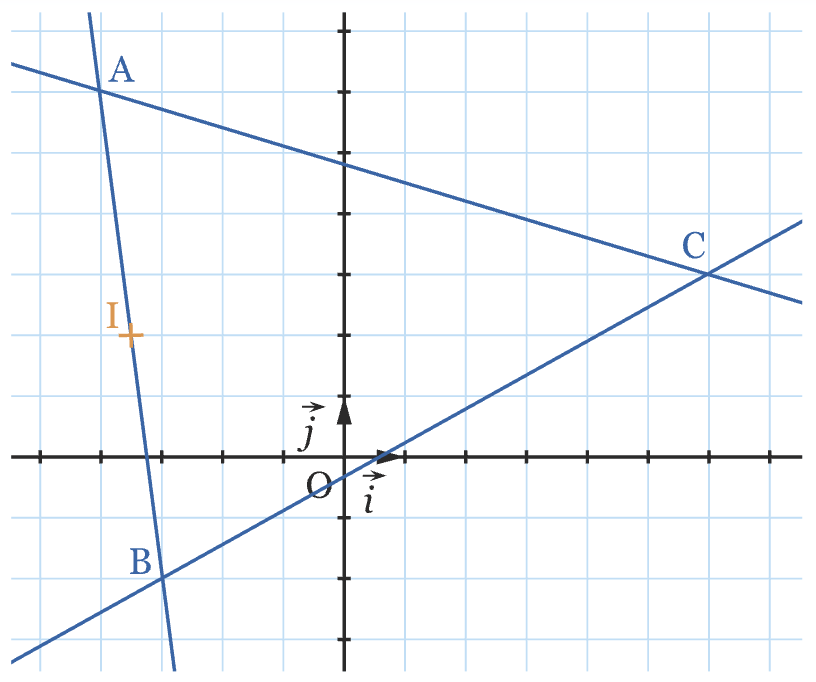
\includegraphics[width=1\textwidth]{fig1.png}
\end{minipage}%

\end{document}
